\documentclass{PoS}

\newcommand{\url}[1]{\href{#1}{#1}}

% Shortcuts
\newcommand{\aap}{AAP}
\newcommand{\pasp}{PASP}
\newcommand{\procspie}{SPIE}

\newcommand{\urlGammapySlack}{\href{https://gammapy.slack.com}{gammapy.slack.com}}
\newcommand{\urlCtaPipe}{\href{https://github.com/cta-observatory/ctapipe}{github.com/cta-observatory/ctapipe}}
\newcommand{\urlPint}{\href{https://github.com/nanograv/PINT}{github.com/nanograv/PINT}}
\newcommand{\urlFermipy}{\href{https://github.com/fermipy/fermipy}{github.com/fermipy/fermipy}}
\newcommand{\urlGammapyDocs}{\href{http://docs.gammapy.org}{docs.gammapy.org}}
\newcommand{\urlErfa}{\href{https://github.com/liberfa/erfa}{github.com/liberfa/erfa}}
\newcommand{\urlSofa}{\href{http://www.iausofa.org}{www.iausofa.org}}
\newcommand{\urlGammapyGithub}{\href{https://github.com/gammapy/gammapy}{github.com/gammapy/gammapy}}
\newcommand{\urlPytest}{\href{https://pytest.org}{pytest.org}}
\newcommand{\urlSphinx}{\href{http://www.sphinx-doc.org}{www.sphinx-doc.org}}
\newcommand{\urlJupyter}{\href{https://jupyter.org}{jupyter.org}}
\newcommand{\urlPypi}{\href{https://pypi.python.org}{pypi.python.org}}
\newcommand{\urlPip}{\href{https://pip.pypa.io}{pip.pypa.io}}
\newcommand{\urlAnacondaGammapy}{\href{https://anaconda.org/astropy/gammapy}{anaconda.org/astropy/gammapy}}
\newcommand{\urlGentooGammapy}{\href{https://packages.gentoo.org/packages/dev-python/gammapy}{packages.gentoo.org/packages/dev-python/gammapy}}
\newcommand{\urlGammapyForum}{\href{https://groups.google.com/forum/\#!forum/gammapy}{groups.google.com/forum/\#!forum/gammapy}}
\newcommand{\urlCtaAck}{\href{http://www.cta-observatory.org/consortium_acknowledgments}{www.cta-observatory.org/consortium\_acknowledgments}}
\newcommand{\urlGithub}{\href{https://github.com}{github.com}}
\newcommand{\urlRtd}{\href{https://readthedocs.org}{readthedocs.org}}
\newcommand{\urlTravis}{\href{https://travis-ci.org}{travis-ci.org}}
\newcommand{\urlAppveyor}{\href{https://appveyor.com}{appveyor.com}}
\newcommand{\urlSlack}{\href{https://slack.com}{slack.com}}

\newcommand{\urlHealpy}{\href{https://healpy.readthedocs.io}{healpy.readthedocs.io}}
\newcommand{\urlRegions}{\href{https://astropy-regions.readthedocs.io}{astropy-regions.readthedocs.io}}
\newcommand{\urlReproject}{\href{https://reproject.readthedocs.io}{reproject.readthedocs.io}}

\title{Gammapy -- A prototype for the CTA science tools}
\ShortTitle{Gammapy -- A prototype for the CTA science tools}

\author{
Christoph Deil$^a$,
Roberta Zanin$^a$,
Julien Lefaucheur$^b$,
Catherine Boisson$^b$,
Bruno Kh\'elifi$^c$,
R\'egis Terrier$^c$,
Matthew Wood$^d$,
Lars Mohrmann$^e$,
Nachiketa Chakraborty$^a$,
Jason Watson$^a$,
Rub\'en L\'opez Coto$^a$,
Stefan Klepser$^f$,
\speaker{Matteo Cerruti}$^g$,
Jean-Philippe Lenain$^g$,
Fabio Acero$^h$,
Arache Djannati-Ata{\"\i}$^c$,
Santiago Pita$^c$,
Zeljka Bosnjak$^i$,
Jos\'e Enrique Ruiz$^j$,
Cyril Trichard$^k$,
Thomas Vuillaume$^l$,
for the CTA Consortium,
Axel Donath$^a$,
Johannes King$^a$,
L\'ea Jouvin$^c$,
Ellis Owen$^m$,
Manuel Paz Arribas$^n$,
Brigitta Sipocz$^o$,
Dirk Lennarz$^p$,
Arjun Voruganti$^a$,
Marion Spir-Jacob$^c$
\\
\llap{$^a$}MPIK, Heidelberg, Germany\\
\llap{$^b$}LUTH, Obs. de Paris/Meudon, France\\
\llap{$^c$}APC/CNRS, Paris, France\\
\llap{$^d$}SLAC National Accelerator Laboratory, US\\
\llap{$^e$}FAU, Erlangen, Germany\\
\llap{$^f$}DESY, Zeuthen, Germany\\
\llap{$^g$}LPNHE, Paris, France\\
\llap{$^h$}CEA/IRFU, Saclay, France\\
\llap{$^i$}University of Rijeka, Croatia\\
\llap{$^j$}IAA-CSIC, Granada, Spain\\
\llap{$^k$}CPPM, Marseille, France\\
\llap{$^l$}LAPP, Annecy-le-Vieux, France\\
\llap{$^m$}UCL-MSSL, Dorking, United Kingdom\\
\llap{$^n$}Humboldt University, Berlin, Germany\\
\llap{$^o$}Cambridge, UK\\
\llap{$^p$}Georgia Tech, Atlanta, US\\
E-mail:
\email{Christoph.Deil@mpi-hd.mpg.de},
\email{Roberta.Zanin@mpi-hd.mpg.de},
\email{julien.lefaucheur@obspm.fr},
\email{catherine.boisson@obspm.fr},
\email{khelifi@apc.in2p3.fr},
}

\abstract{

Gammapy is a Python package for high-level gamma-ray data analysis built on
Numpy, Scipy and Astropy. It enables to analyse gamma-ray data and to create 
sky images, spectra and lightcurves, from event lists and instrument response 
information, as to determine the position, morphology
and spectra of gamma-ray sources.

So far Gammapy has mostly been used to analyse data from H.E.S.S. and Fermi-LAT,
and is now being used for the simulation and analysis of observations from
the Cherenkov Telescope Array (CTA). We have proposed Gammapy as a prototype for
the CTA science tools. This contribution gives an overview of the Gammapy
package and shows an analysis application example with simulated CTA data.

}

\FullConference{35th International Cosmic Ray Conference --- ICRC2017\\
		10--20 July, 2017\\
		Bexco, Busan, Korea}


\begin{document}

\section{Introduction}
\label{sec:intro}

% CTA and CTA science tools introduction
The Cherenkov Telescope Array (CTA) will observe the sky in very-high-energy
(VHE, E > 20$\,$GeV) gamma-ray light soon. CTA will consist of large telescope
arrays at two sites, one in the southern (Chile) and one in the northern (La
Palma) hemisphere. It will perform surveys of large parts of the sky, targeted
observations on Galactic and extra-galactic sources, and more specialized
analyses like a measurement of charged cosmic rays, constraints on the
intergalactic medium opacity for gamma-rays and a search for dark matter.
Compared to current Cherenkov telescope arrays such as H.E.S.S., VERITAS or
MAGIC, CTA will have a much improved detection area, angular and energy
resolution, improved signal/background classification and sensitivity. CTA is
expected to operate for thirty years, and all astronomers will have access to
CTA high-level data, as well as CTA science tools (ST) software. The ST can be
used for example to generate sky images and to measure source properties such as
morphology, spectra and light curves, using event lists as well as instrument
response function (IRF) and auxiliary information as input. 

% What is Gammapy?
Gammapy is a prototype for the CTA ST, built on the scientific Python stack and
Astropy \cite{astropy}, optionally using Sherpa \cite{sherpa2001, sherpa2009,
sherpa2011} or other packages for modeling and fitting (see
Figure~\ref{fig:stack}). A 2\hbox{-}dimensional analysis of the sky images 
for source detection and morphology fitting, followed by spectral analysis, was first 
implemented. A 3\hbox{-}dimensional analysis with a simultaneous spatial and spectral model of
the gamma-ray emission, as well as background (called ``cube analysis'' in the
following) is under development.
% Existing studies using Gammapy
A first study comparing spectra obtained with the classical 1D analysis and the
3D cube analysis using point source observations with H.E.S.S. is presented in \cite{lea}. Further
developments and verification using data from existing Cherenkov telescope
arrays such as H.E.S.S. and MAGIC, as well as simulated CTA data is ongoing.
% Gammapy use in CTA
Gammapy is now used for scientific studies with existing ground-based
gamma-ray telescopes \cite{hgps, shells}, the Fermi-LAT space telescope
\cite{owen2015}, as well as for CTA \cite{julien, roberta, cyril}.

\begin{figure}[t]
\centering
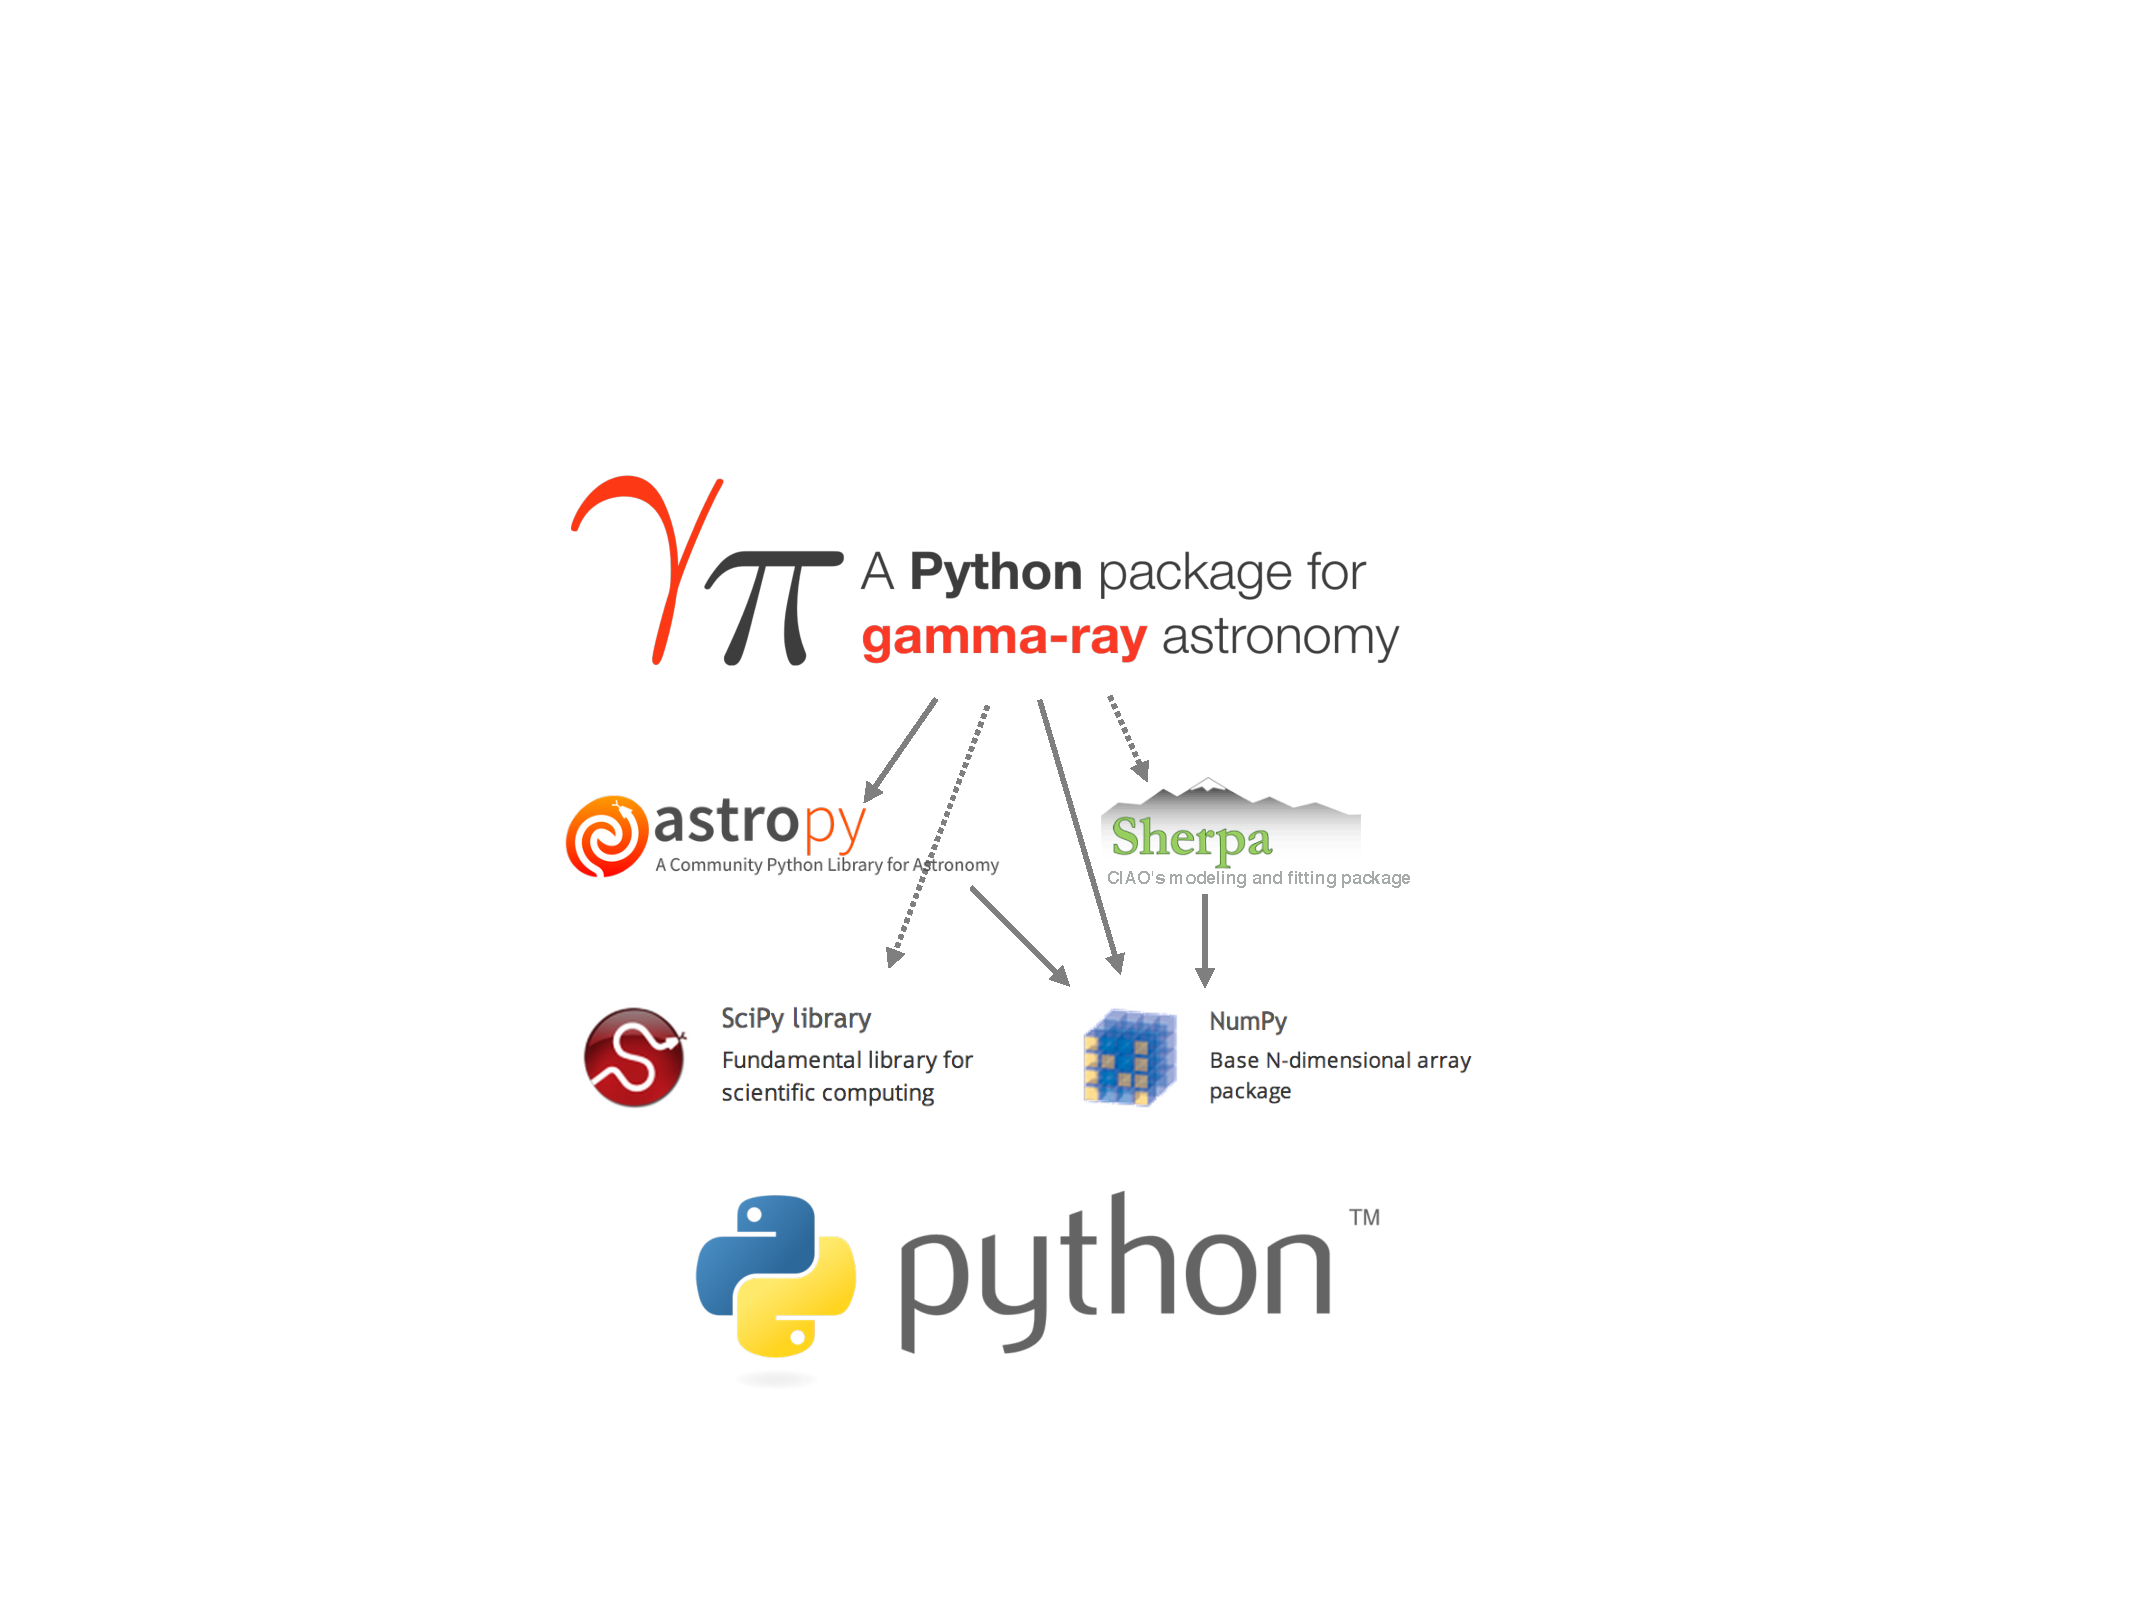
\includegraphics[width=0.5\textwidth]{figures/gammapy-stack}
\caption{
The Gammapy software stack. Required dependencies (Python, Numpy and Astropy)
are illustrated with solid arrows, optional dependencies (Scipy and Sherpa) with
dashed arrows.
}
\label{fig:stack}
\end{figure}

% Outline of this paper
In this writeup we focus on the software and technical aspects of Gammapy.We
start with a brief overview of the context in Section~\ref{sec:context},
followed by a description of the Gammapy package in Section~\ref{sec:package},
the Gammapy project in Section~\ref{sec:project} and finally our conclusions
concerning Gammapy as as CTA science tool prototype in
Section~\ref{sec:conclusions}.

\section{Context}
\label{sec:context}

% Python, Numpy, Astropy
Prior to Gammapy, in 2011/2012, a collection of Python scripts for the analysis
of IACT data was released as a first test of open-source VHE data analysis
software: ``PyFACT: Python and FITS Analysis for Cherenkov Telescopes''
\cite{pyfact}. This project is not updated anymore, but it was the first 
implementation of our idea to build a CTA science tools package based on 
Python and using Numpy and Scipy, during the first development stages of the CTA 
project. In 2011, the astronomical Python community came
together and created the Astropy project and package \cite{astropy}, which is a
key factor making Python the most popular language for astronomical research
codes (at least according to this informal analysis \cite{perry} and survey
\cite{momcheva2015}). Gammapy is an Astropy affiliated package, which means that
where possible it uses the Astropy core package instead of duplicating its
functionality, as well as having a certain quality standard such as having
automated tests and documentation for the available functionality. In recent
years, several other packages have adopted the same approach, to build on
Python, Numpy and Astropy. To name just a few, there is ctapipe (\urlCtaPipe),
the prototype for the low-level CTA data processing pipeline (up to the creation
of lists of events and IRFs); Naima for modeling the non-thermal spectral energy
distribution of astrophysical sources \cite{naima}; PINT, a new software for
high-precision pulsar timing (\urlPint), and Fermipy (\urlFermipy), a Python
package that facilitates analysis of data from the Large Area Telescope (LAT)
with the Fermi Science Tools and adds some extra functionality.

We note that many other astronomy projects have chosen Python and Astropy as the
basis both for their data calibration and reduction pipelines and their science
tools. Some prominent examples are the Hubble space telescope (HST)
\cite{hubble}, the upcoming James Webb Space Telescope (JWST) \cite{jwst} and
the Chandra X-ray observatory \cite{sherpa2001, chandra}. Even projects like
LSST that started their analysis software developments before Astropy existed
and are based on C++/SWIG are now actively working towards making their software
interoperable with Numpy and Astropy, to avoid duplication of code and
development efforts, but also to reduce the learning curve for their science
tool software (since many astronomers already are using Python, Numpy and
Astropy) \cite{lsst}.

% Comparison to Gammalib, ctools
% Another open-source package that has been proposed as a prototype for the CTA
% science tools is Gammalib/ctools \cite{ctools}. Gammalib is a C++ library with
% SWIG Python wrappers that doesn't have any dependencies besides CFITSIO, instead
% implementing the functionality needed from scratch. ctools is a set of command
% line tools, following the FTOOLs model of using FITS files as input and output
% and being able to chain them into analysis chains using Python. Concerning
% analysis methods, Gammalib/ctools is supporting binned and unbinned likelihood
% analysis and implemented ``cube analysis'' first, adding support for ``classical
% analysis'' now (the other way around compared to Gammapy).

% The choice for the official CTA science tools, supported and distributed by the
% CTA observatory, has not been made yet; at this time both Gammapy and
% Gammalib/ctools are open-source codes being used for CTA as well as exiting
% gamma-ray telescopes. 

% Open data formats
For current ground-based IACTs, data and software are mostly private to the
collaborations operating the telescopes. CTA will be, for the first time in VHE
gamma-ray astronomy, operated as an open observatory. This implies fundamentally
different requirements for the data formats and software tools. Along this path,
the current experiments, H.E.S.S., MAGIC and VERITAS, have started converting
their data to FITS format, yet relying on different (some private, some open)
analysis tools, and many slightly different ways to store the same information in
FITS files appeared. The CTA high-level data model and data format specifications 
are currently being written and will give a framework to the current experiments
to store data. The methods to link events to IRFs still have to be extended to 
support multiple event types and the IRF and background model formats will have to be 
extended to be more precise \cite{opendata}. The Gammapy team is participating 
in and contributing to the effort to prototype and find a good high-level data 
model and formats for CTA.


% One issue noticed in the past years was that in the current situation of having
% multiple telescopes converting their data to FITS format and multiple science
% tools, it became necessary to write down the details of the data formats being
% used. At this time, the data formats used in existing science tool codes
% (Gammapy, Gammalib/ctools and partly also others, like Fermipy, 3ML \cite{3ml}
% or Naima \cite{naima}) are to a large degree the same, although one has to
% mention that the development of the DL3 data model and formats is work in
% progress, and especially the IRF formats and DL3 data linking of events to IRFs
% to support multiple event types will have to be extended \cite{opendata}, a
% process Gammapy is participating in and contributing to.


\section{Gammapy package}
\label{sec:package}

Gammapy offers the high-level analysis tools to generate science results (images, spectra,
light curves and source catalogs) based on input data consisting of 
reconstructed events (with an arrival direction and an energy) that are 
classified according to their types (e.g. gamma-like, cosmic-ray-like). 
In the data processing chain of CTA, the reconstruction and classification 
of events are realized by an other Python package, ctapipe\footnote{\urlCtaPipe}. Data are stored in FITS format. 
The high-level analysis consists on: 
\vspace{-0.3cm}
\begin{itemize}
\setlength\itemsep{-0.5em}
\item selection of a data cube (energy and positions) around a sky position from all event
lists,
\item computation of the corresponding exposure,
\item estimation the background directly from the data (e.g. with a RingBackground model \cite{berge}) 
or from a model (template to be built on real data beforehand),
\item creation of sky images (signal, background, significance, etc) and morphology fitting,
\item spectrum measurement with a 1D analysis or with a 3D analysis by adjusting both spectral and spatial shape of gamma-ray sources,
\item computation of light-curves and phasograms, search for transient signal,
\item derivation of a catalog of excess peaks (or a source catalog).

\end{itemize}
\vspace{-0.28cm}
For such an analysis, Gammapy is using the IRFs produced by the ctapipe  package and 
processes them precisely to get an accurate estimation of high-level astrophysical quantities.


The Gammapy code base is structured into several sub-packages dedicated to specific classes 
where each of the packages bundle corresponding functionality in a namespace 
(e.g. data and observation handling "gammapy.data", IRF functionnality "gammapy.irf, spectrum 
estimation and modeling "gammapy.spectrum"...).  The
Gammapy features are described in detail in the Gammapy documentation
(\urlGammapyDocs) and many examples given in the tutorial-style Jupyter
notebooks, as well as in \cite{gammapy-icrc2015}. Figure~\ref{fig:app} shows one result of the ``CTA data analysis with Gammapy''
notebook: a significance sky image of the Galactic center region using 1.5~hours
of simulated CTA data. The background was estimated using the ring background
estimation technique, and peaks above 5~sigma are shown with white circles. For examples of CTA science
studies using Gammapy, we refer you to other posters presented at this
conference: Galactic survey \cite{roberta}, PeVatrons \cite{cyril} and
extra-galactic sources \cite{julien}. Several other examples using real data
from H.E.S.S. and Fermi-LAT, as well as simulated data for CTA can be found via
\urlGammapyDocs\ by following the link to ``tutorial notebooks''.
 
The Gammapy Python package is primarily built on Numpy \cite{numpy}, and Astropy
\cite{astropy} as core dependencies. Data is stored in Numpy arrays or objects
such as {\it astropy.coordinates.SkyCoord} or {\it astropy.table.Table} that
hold Numpy array data members. Numpy provides many functions for array-oriented
computing and numerics, and Astropy provides astronomy-specific functionality.
The Astropy functionality most commonly used in Gammapy is {\it astropy.io.fits}
for FITS data I/O, {\it astropy.table.Table} as a container for tabular data
(e.g. event lists, but also many other things like spectral points or source
catalogs), {\it astropy.wcs.WCS} for world coordinate systems mapping pixel to
sky coordinates, as well as {\it astropy.coordinates.SkyCoord} and {\it
astropy.time.Time} objects to represent sky coordinates and times. Astropy.coordinates 
as well as astropy.time are built on ERFA (https://github.com/liberfa/erfa), the
open-source variant of this IAU Standards of Fundamental Astronomy (SOFA) 
C library (http://www.iausofa.org/). In Gammapy,
we use {\it astropy.units.Quantity} objects extensively, where a quantity is a
Numpy array with a unit attached, supporting arithmetic in computations and
making it easier to read and write code that does computations involving
physical quantities.

As an example, a script that generates a counts image from an event list using Gammapy
is shown in Figure~\ref{fig:code_example}. The point we want to make here is
that it is possible to efficiently work with events and pixels and to implement
algorithms from Python, by storing all data in Numpy arrays and processing via
calls into existing C extensions in Numpy and Astropy. E.g. here {\it EventList}
stores the RA and DEC columns from the event list as Numpy arrays, and {\it
SkyImage} the pixel data as well, and {\it image.fill(events)}, and all
processing happens in existing C extensions implemented or wrapped in Numpy and
Astropy. In this example, the {\it read} and {\it write} methods call into {\it
astropy.io.fits} which calls into CFITSIO (\cite{cfitsio}), and the {\it
image.fill(events)} method calls into {\it astropy.wcs.WCS} and WCSLib
(\cite{wcslib}) as well as {\it numpy.histogramdd}. 

\begin{figure}[t]
\centering
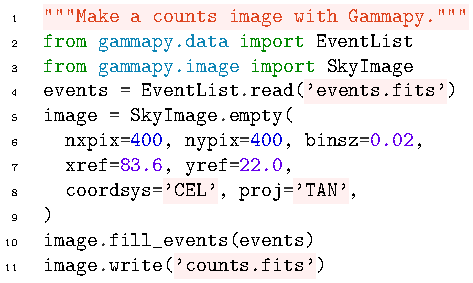
\includegraphics[width=0.5\textwidth]{examples/code_events_image}
\caption{An example script using Gammapy to make a counts image from an event list. This
is used in Section~\protect\ref{sec:package} to explain how Gammapy achieves efficient
processing of event and pixel data from Python: all data is stored in Numpy
arrays and passed to existing C extensions in Numpy and Astropy.}
\label{fig:code_example}
\end{figure}

Gammapy aims to be a base package on which other more specialized packages such
as Fermipy (\urlFermipy) for Fermi-LAT data analysis or Naima \cite{naima} for
the modeling of non-thermal spectral energy distributions of astrophysical
sources can build.
% \footnote{The relation of Gammapy to ctapipe (\urlCtaPipe)
% isn't clear yet; at this time neither package imports functionality from the
% other, and some duplication of functionality exists (e.g. for CTA sensitivity
% computation).}.
For this reason we avoid introducing new required dependencies
besides Numpy and Astropy. That said, Gammapy does import the following optional
dependencies to provide extra functionality (sorted in the order of how common
their use is within Gammapy). Scipy \cite{scipy} is used for integration and
interpolation, Matplotlib \cite{matplotlib} for plotting and Sherpa
\cite{sherpa2001, sherpa2009, sherpa2011} for modeling and fitting. In addition,
the following packages are used at the moment for functionality that we expect
to become available in the Astropy core package within the next year: regions
(\urlRegions) to handle sky and pixel regions, reproject (\urlReproject) for
reprojecting sky images and cubes and healpy (\urlHealpy) for HEALPix data
handling. 

%We note that with the Gammapy approach, a huge eco-system of scientific Python
%as well as Astropy-affiliated packages is available for advanced users, to
%implement analysis methods for special use cases (e.g. sky or background models,
%IRF handling or likelihood or Bayesian analysis methods) in an efficient way in
%pure Python packages or scripts. To name just a few that we have seen used in
%conjunction with Gammapy so far (by users, not within the Gammapy package
%itself): pandas, scikit-image, scikit-learn, iminuit, emcee as well as Fermipy,
%Naima and PINT.


\begin{figure}[t]
\centering
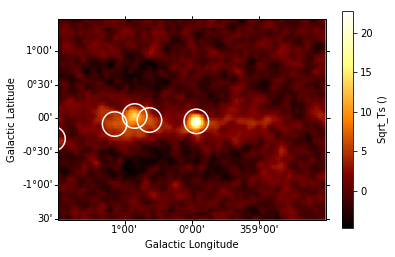
\includegraphics[width=0.7\textwidth]{figures/gammapy_example_sky_image.png}
\caption{
Application example: significance image for the Galactic centre region using
1.5~hours of simulated CTA data.  White circles are peaks above 5~sigma.
}
\label{fig:app}
\end{figure}

\section{Gammapy project}
\label{sec:project}

In this section we describe the current setup of the Gammapy project. We are using the common tools and services for Python open-source projects for software
development, code review, testing, documentation, package distribution and user
support.

Gammapy development happens on Github (\urlGammapyGithub). We make extensive use
of the pull request system to discuss and review code contributions. For testing
we use pytest (\urlPytest), for continuous integration Travis-CI (Linux and Mac)
as well as Appveyor (Windows). For documentation Sphinx (\urlSphinx), for
tutorial-style documentation Jupyter notebooks (\urlJupyter) are used.

Gammapy is distributed and installed in the usual way for Python packages. Each
stable release is uploaded to the Python package index (\urlPypi), and
downloaded and installed by users via {\it pip install gammapy} (\urlPip).
Binary packages for conda are available via the conda Astropy channel
(\urlAnacondaGammapy) for Linux, Mac and Windows, which conda users can install
via {\it conda install gammapy -c astropy}. Binary packages for the Macports
package manager are also available, which users can install via {\it port
install gammapy}. At this time, Gammapy is also available as a Gentoo Linux
package (\urlGentooGammapy) and a Debian Linux package is in preparation.

For Gammapy developer team communication we use Slack (\urlGammapySlack). A
public mailing list for user support and discussion is available
(\urlGammapyForum). Two face-to-face meetings for Gammapy were organized so far,
the first on in June 2016 in Heidelberg as a coding sprint for developers only,
the second on in February 2017 in Paris as a workshop for both Gammapy users and
developers.

% Note that the current setup described in this section is different from what it
% will be if Gammapy is chosen to be the or part of the CTA science tools, since
% CTA will set up their own systems for software development, maintenance,
% testing, documentation, issue tracking, software distribution and user support.

{\bf BKH: Add a status here... on the functionalities... done, under dev., to be dev.}

\section{Conclusions}
\label{sec:conclusions}

In the past two years, we have developed Gammapy as an open-source analysis
package for existing gamma-ray telescope and as a prototype for the CTA science
tools. Gammapy is a Python package, consisting of functions and classes that can
be used as a flexible and extensible toolbox to implement and execute high-level
gamma-ray data analyses.

We find that the Gammapy approach, to build on the powerful and well-tested
Python packages Numpy and Astropy, brings large benefits: a small codebase that
is focused on gamma-ray astronomy in a single high-level language is easy to
understand and maintain. It is also easy to modify and extend as new use cases
arise, which is important for CTA, since it can be expected that the modeling of
the instrument, background and astrophysical emission, as well as the analysis
method in general (e.g. likelihood or Bayesian statistical methods) will evolve
and improve over the next decade. Last but not least, the Gammapy approach is
inherently collaborative {\bf CB TO BE CHECKED }($~$30 people community of developers){\bf CB }, 
sharing development effort as well as know-how with the larger astronomical community, 
that to a large degree already has adopted
Numpy and Astropy as the basis for astronomical analysis codes in the past 5
years.

\section{Acknowledgements}
\label{sed:acknowledgements}

This work was conducted in the context of the CTA Consortium. We gratefully
acknowledge financial support from the agencies and organizations listed here:\\
\urlCtaAck

We would like to thank the Scientific Python and specifically the Astropy
community for providing their packages which are invaluable to the development
of Gammapy, as well as tools and help with package setup and continuous
integration, as well as building of conda packages.

We thank the GitHub (\urlGithub) team for providing us with an excellent free
development platform, ReadTheDocs (\urlRtd) for free documentation hosting,
Travis (\urlTravis) and Appveyor (\urlAppveyor) for free continuous integration
testing, and Slack (\urlSlack) for a free team communication channel.

\bibliography{gammapy-icrc2017}
\bibliographystyle{JHEP}

\end{document}
